% Рисуночки
\section{Конструкторская часть}
\subsection*{Описания алгоритмов}

\hspace{1.25cm}
На основании теоретических измышлений были разработаны алгоритмы, вычисляющие расстояние Левенштейна и Дамерау-Левенштейна тремя способами: матричным, рекурсивным и рекурсивно-матричным. Блок-схемы этих алгоритмов приведены ниже.

\begin{figure}[H]
    \centering
    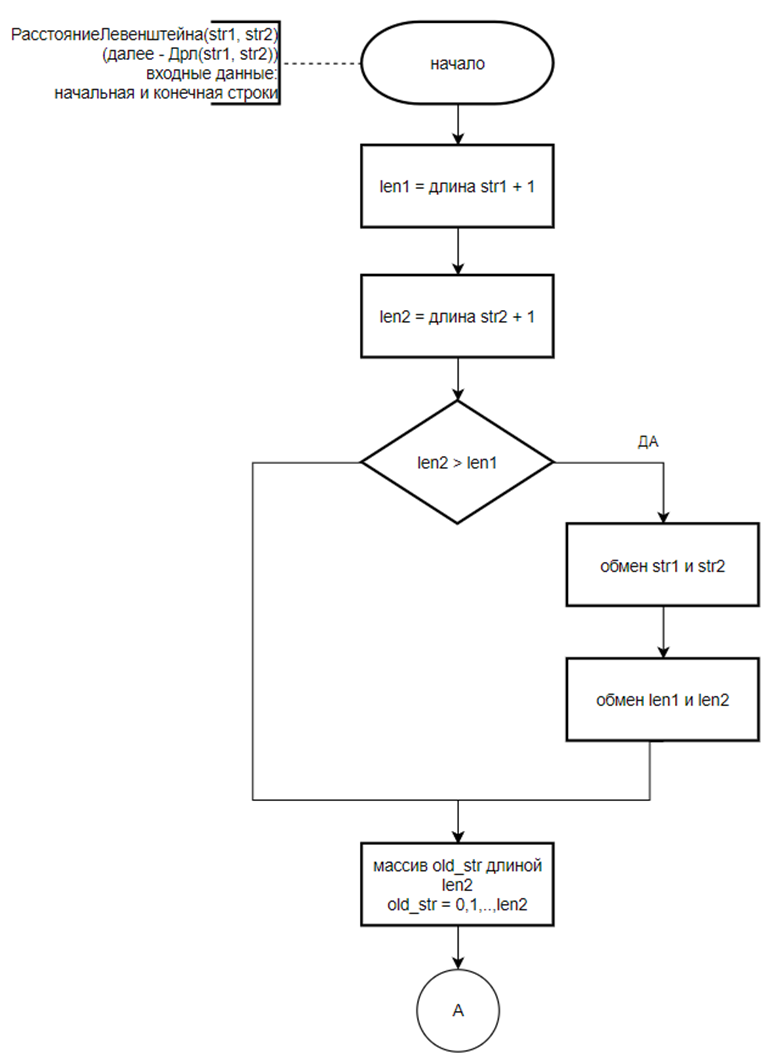
\includegraphics[width=0.9\textwidth]{img/block_1_1_1.png}
    \caption{Блок-схема алгоритма Левенштейна (матричная реализация)}
\end{figure}

\begin{figure}[H]
    \centering
    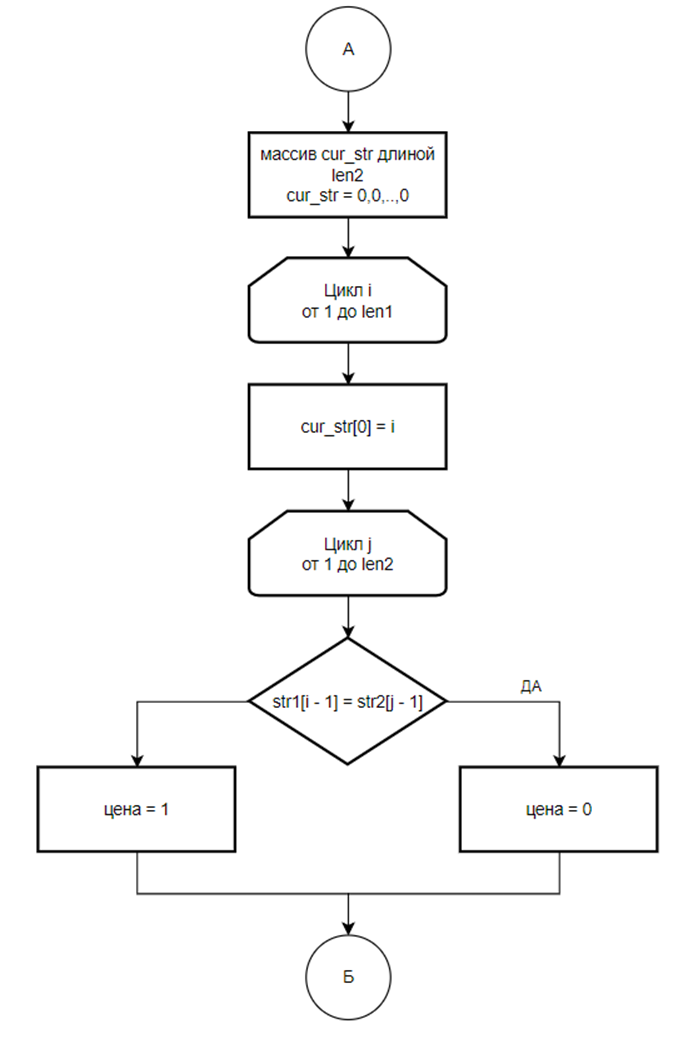
\includegraphics[width=0.9\textwidth]{img/block_1_1_2.png}
    \caption{Блок-схема алгоритма Левенштейна (матричная реализация) (продолжение)}
\end{figure}

\begin{figure}[H]
    \centering
    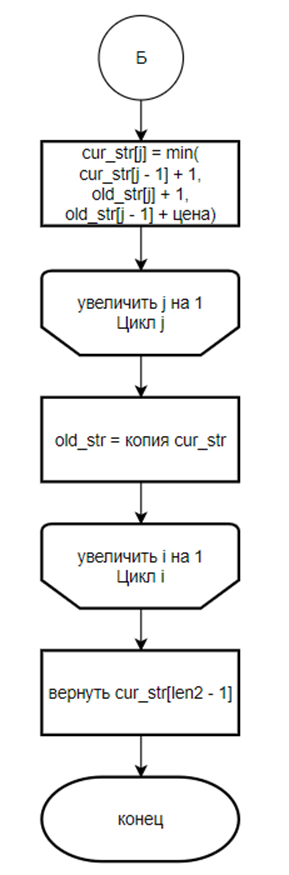
\includegraphics[width=0.4\textwidth]{img/block_1_1_3.png}
    \caption{Блок-схема алгоритма Левенштейна (матричная реализация) (продолжение (2))}
\end{figure}

\begin{figure}[H]
    \centering
    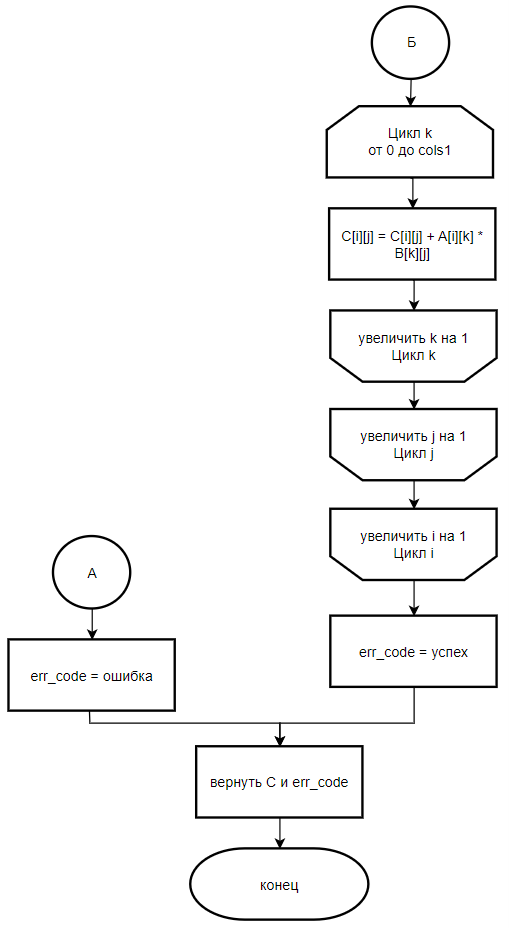
\includegraphics[width=1.1\textwidth]{img/block_1_2.png}
    \caption{Блок-схема алгоритма Левенштейна (рекурсивная реализация)}
\end{figure}

\begin{figure}[H]
    \centering
    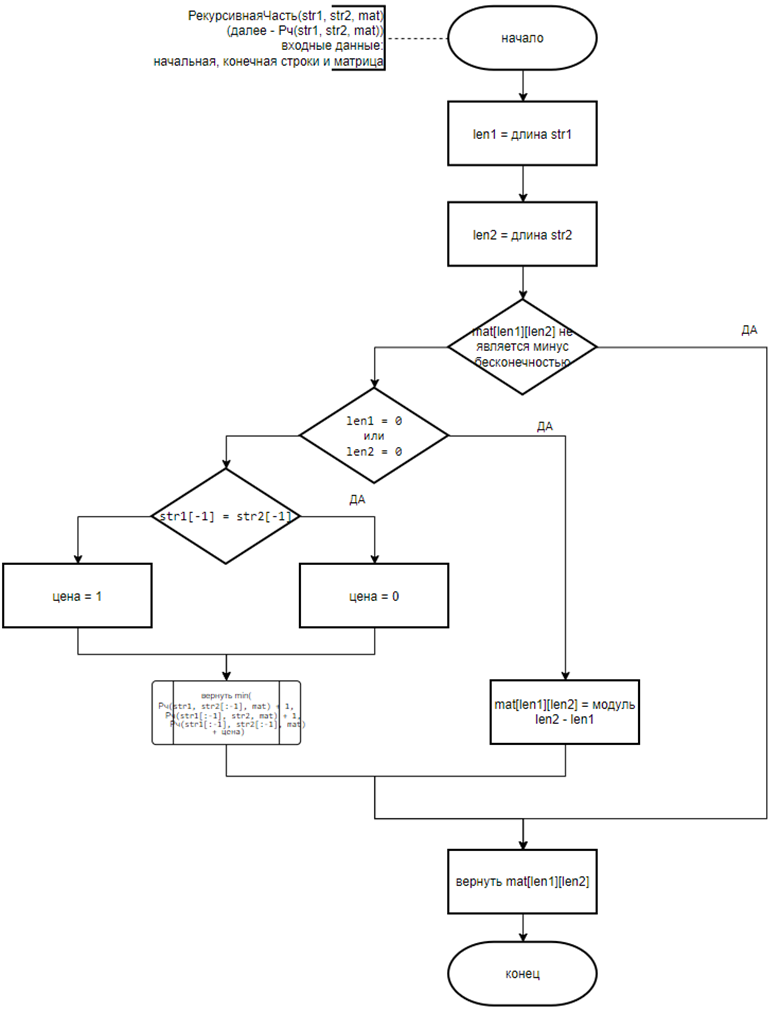
\includegraphics[width=1.05\textwidth]{img/block_1_3_1.png}
    \caption{Блок-схема алгоритма Левенштейна (рекурсивно-матричная реализация)}
\end{figure}

\begin{figure}[H]
    \centering
    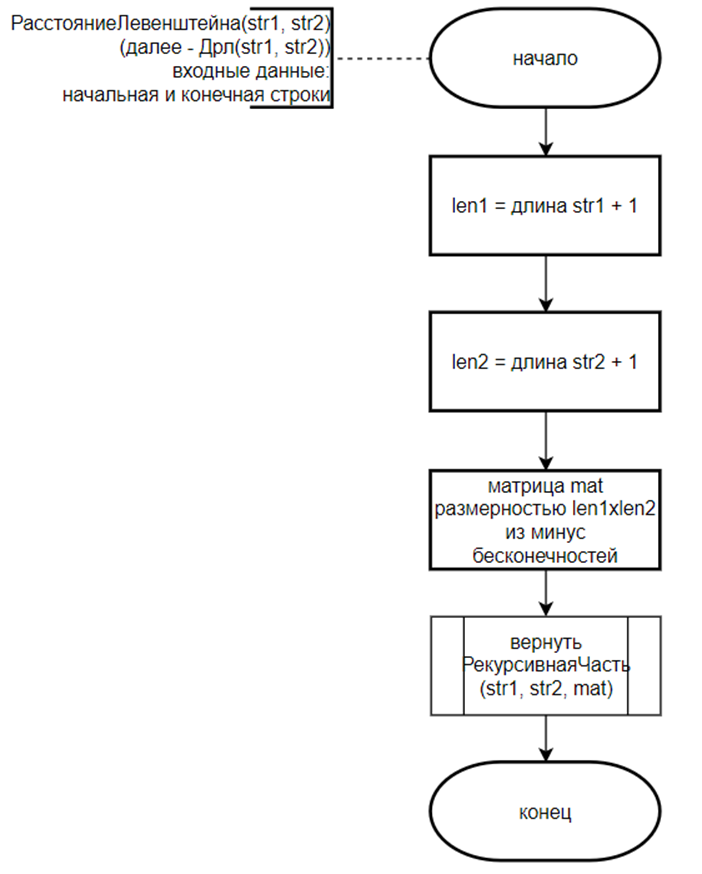
\includegraphics[width=0.9\textwidth]{img/block_1_3_2.png}
    \caption{Блок-схема алгоритма Левенштейна (рекурсивно-матричная реализация\\(продолжение))}
\end{figure}

\begin{figure}[H]
    \centering
    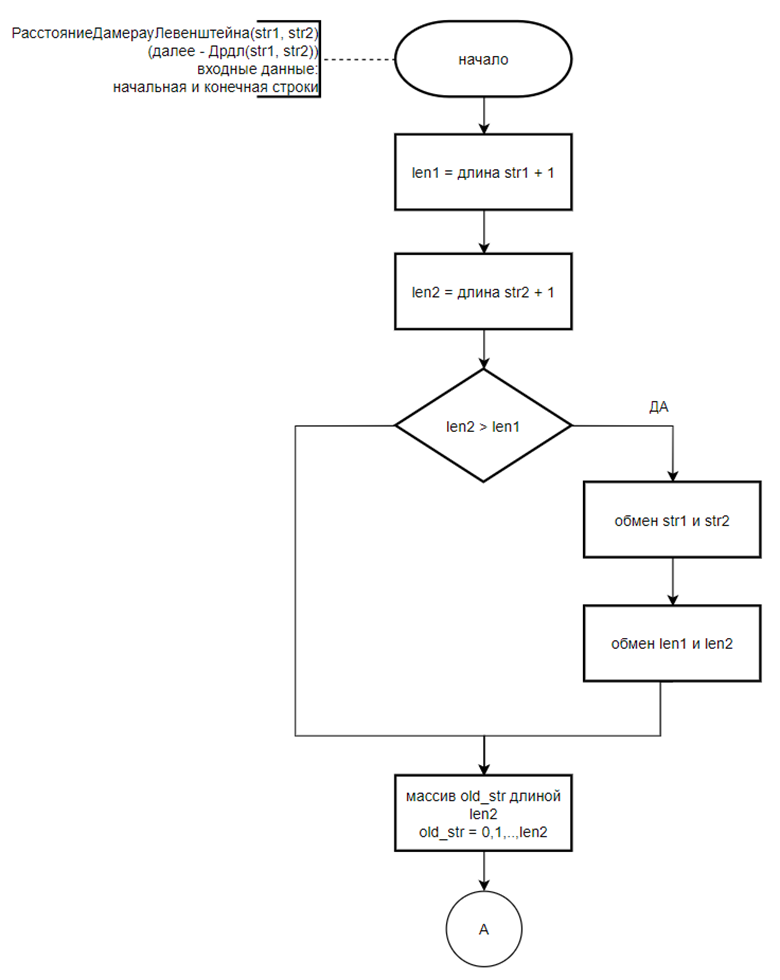
\includegraphics[width=1.05\textwidth]{img/block_2_1_1.png}
    \caption{Блок-схема алгоритма Дамерау-Левенштейна (матричная реализация)}
\end{figure}

\begin{figure}[H]
    \centering
    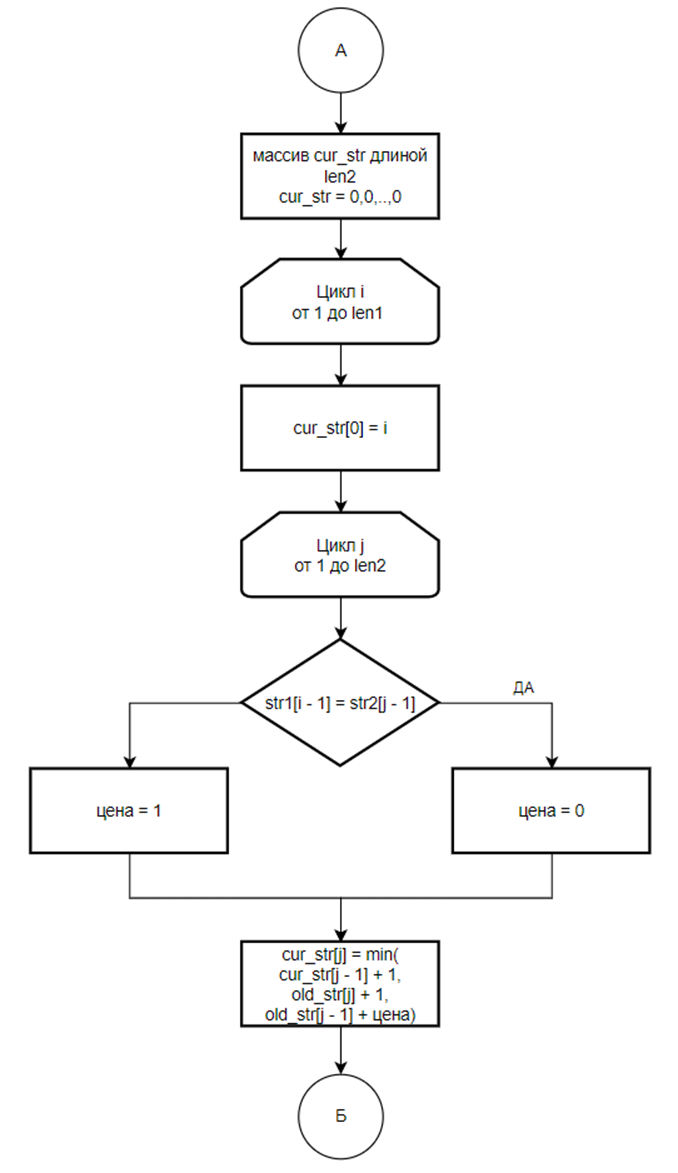
\includegraphics[width=0.8\textwidth]{img/block_2_1_2.png}
    \caption{Блок-схема алгоритма Дамерау-Левенштейна (матричная реализация)\\ (продолжение)}
\end{figure}

\begin{figure}[H]
    \centering
    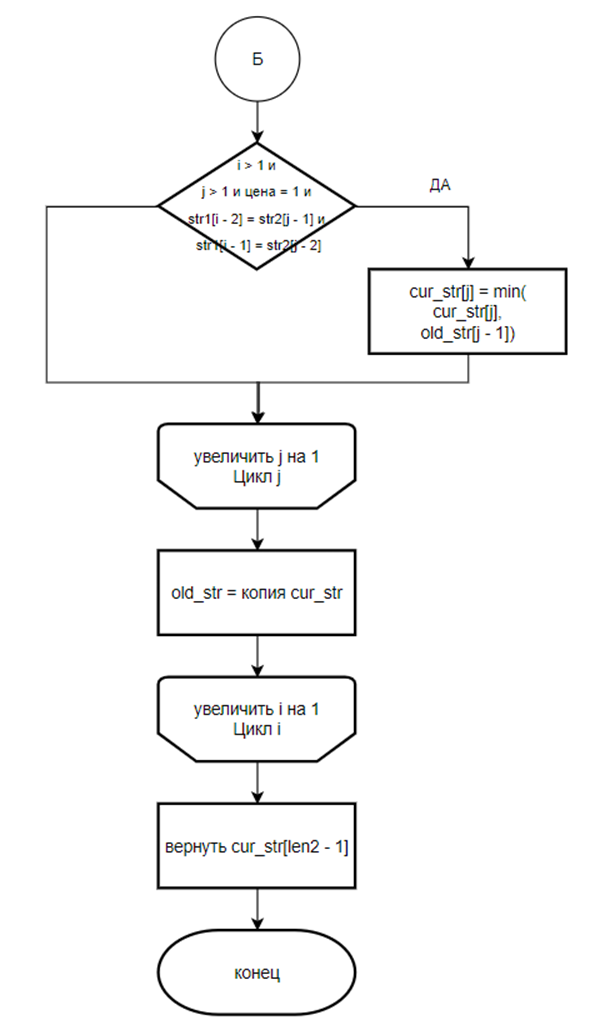
\includegraphics[width=0.8\textwidth]{img/block_2_1_3.png}
    \caption{Блок-схема алгоритма Дамерау-Левенштейна (матричная реализация)\\ (продолжение (2))}
\end{figure}

\begin{figure}[H]
    \centering
    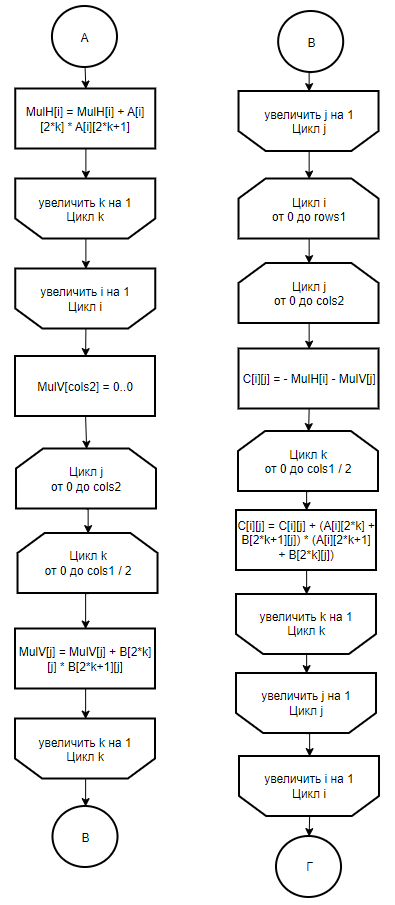
\includegraphics[width=0.95\textwidth]{img/block_2_2.png}
    \caption{Блок-схема алгоритма Дамерау-Левенштейна (рекурсивная реализация)}
\end{figure}

\begin{figure}[H]
    \centering
    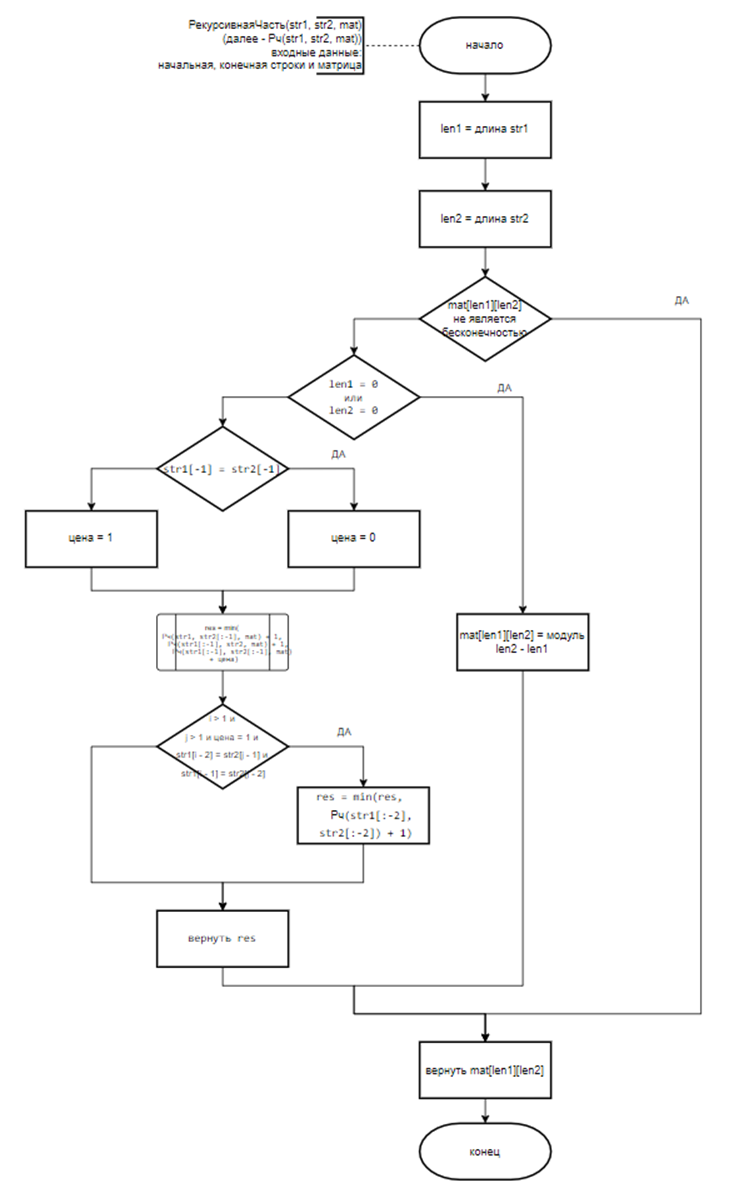
\includegraphics[width=0.93\textwidth]{img/block_2_3_1.png}
    \caption{Блок-схема алгоритма Дамерау-Левенштейна (рекурсивно-матричная\\ реализация)}
\end{figure}

\begin{figure}[H]
    \centering
    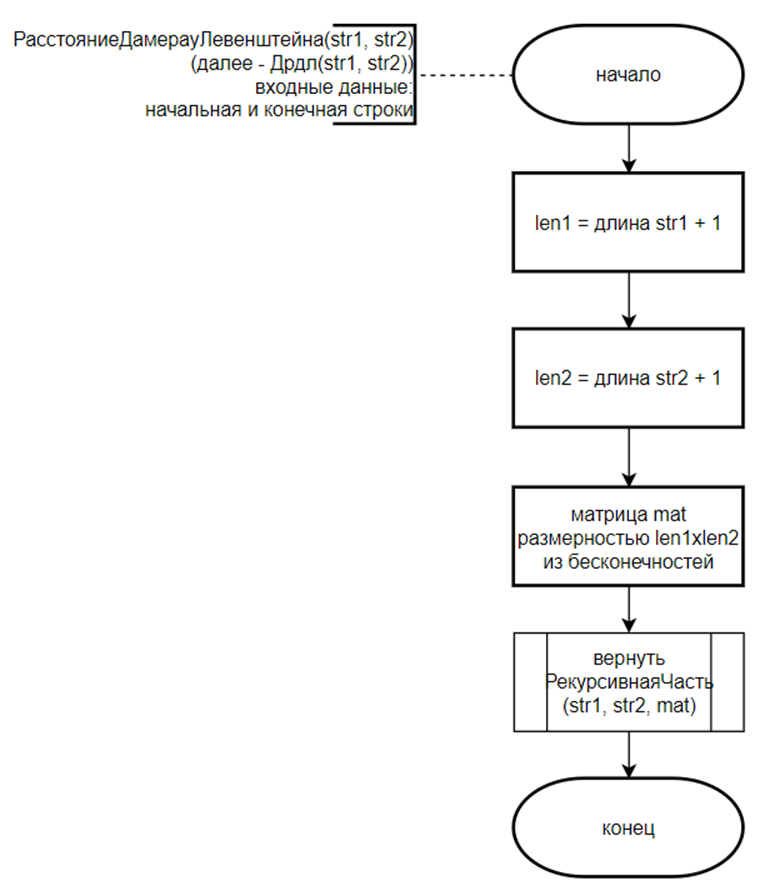
\includegraphics[width=1\textwidth]{img/block_2_3_2.png}
    \caption{Блок-схема алгоритма Дамерау-Левенштейна (рекурсивно-матричная\\ реализация (продолжение))}
\end{figure}
\newpage